\documentclass[aspectratio=43]{beamer}
\usepackage[latin1]{inputenc}
\usepackage{amsmath}
\usepackage{amsfonts}
\usepackage{amssymb}
\usepackage{makeidx}
\usepackage{graphicx}
\usepackage{array}

% Customization
\mode<presentation>{
\usetheme{CambridgeUS}
\usecolortheme{dolphin}
\setbeamertemplate{navigation symbols}{}
}

%\setbeamertemplate{footline}[frame number]

%TikZ diagrams
\usepackage{tikz}
\usetikzlibrary{patterns}
\usetikzlibrary{arrows,shapes}
\usetikzlibrary{shapes.multipart}
\usetikzlibrary{trees}
\usetikzlibrary{shapes.geometric}
\usetikzlibrary{matrix,arrows}
\usetikzlibrary{positioning}
\usetikzlibrary{calc,through}
\usetikzlibrary{decorations.pathreplacing}
\usepackage{pgffor}

% Define colors
\definecolor{darkgreen}{rgb}{0.0, 0.5, 0.13}
\definecolor{darkblue}{rgb}{0.0, 0.0, 0.55}
\definecolor{darkred}{rgb}{0.55, 0.0, 0.0}

% For using TikZ
\usetikzlibrary{decorations.pathmorphing}
\usetikzlibrary{decorations.markings}
\tikzset{
	vector/.style={decorate, decoration={snake,amplitude=3pt}, draw},
	gluon/.style={decorate, decoration={coil,amplitude=2.5pt},draw},
	provector/.style={decorate, decoration={snake,amplitude=2.5pt}, draw},
	antivector/.style={decorate, decoration={snake,amplitude=-2.5pt}, draw},
	fermion/.style={draw=black, postaction={decorate},
		decoration={markings,mark=at position .55 with {\arrow[draw=black,thick]{>}}}},
	fermionbar/.style={draw=black, postaction={decorate},
		decoration={markings,mark=at position .55 with {\arrow[draw=black,thick]{<}}}},
	fermionnoarrow/.style={draw=black},
	gluon/.style={decorate, draw=black,
		decoration={coil,amplitude=2.5pt, segment length=3pt}},
	gluon2/.style={decorate, draw=black,
		decoration={coil,amplitude=1.75pt, segment length=2.75pt}},
	scalar/.style={dashed,draw=black, postaction={decorate},
		decoration={markings,mark=at position .55 with {\arrow[draw=black]{>}}}},
	scalarbar/.style={dashed,draw=black, postaction={decorate},
		decoration={markings,mark=at position .55 with {\arrow[draw=black]{<}}}},
	scalarnoarrow/.style={dashed,draw=black},
	electron/.style={draw=black, postaction={decorate},
		decoration={markings,mark=at position .55 with {\arrow[draw=black]{>}}}},
	bigvector/.style={decorate, decoration={snake,amplitude=4pt}, draw},
}

% Blocks
\tikzstyle{block} = [draw, rectangle, minimum height = 3em, rounded corners, minimum width = 4em]
\tikzstyle{block2} = [draw, rectangle, minimum height = 3em, rounded corners, minimum width = 7em]
\tikzstyle{circle} = [draw, circle, radius = 1.5]
\tikzstyle{arrow} = [thick,->]
%************************************************************************************************************

% Title and author
\title[GP for theory uncertainties]{Machine Learning for the precision determination of Parton Distribution Functions}
\author{\textbf {Jes\'us Urtasun Elizari}}
%\institute{\textbf {University of Milan}}
\date{Milan, September 2020}

\begin{document}

% Front slide
\begin{frame}

	%\maketitle
	\vspace{1.0 cm}
	
	\center{\color{blue}Gaussian Process for the estimation of theory uncertainties}
	
	\vspace{0.25 cm}
	\center{Jes\'us Urtasun Elizari}
	\center{Italian Physical Society - Milan, September 2020}

	\begin{figure}
		\minipage{1\textwidth}
		
\includegraphics[width = 3.0 cm]{plots/unimi.png}
		\hfill
		
\includegraphics[width = 3.0 cm]{plots/n3pdf.png}
		\hfill
		
\includegraphics[width = 3.0 cm]{plots/erc.png}
		\endminipage
	\end{figure}

	\vspace{1.0 cm}
	
	{\scriptsize \color{blue} This project has received funding from the European Union$'$s Horizon 2020 research and innovation program under grant agreement No 740006.}

\end{frame}

% Introduction
\begin{frame}

	\frametitle{Outline}
	
	\begin{enumerate}
		\item {\color{blue}QCD in a nutshell}
		\begin{itemize}
			\item The Standard Model of particle physics
			\item LHC physics and theory uncertainties
			\item Factorization theorem
		\end{itemize}
		\item {\color{blue}Machine Learning}
		\begin{itemize}
			\item Motivation for Machine Learning
			\item Neural Networks $\&$ general strategy
		\end{itemize}
		\item {\color{blue}Gaussian Process and theory uncertainties}
		\begin{itemize}
			\item The N3PDF project
			\item Kernel based methods
			\item Results $\&$ Conclusions
		\end{itemize}
	\end{enumerate}
	
\end{frame}

% The Standard model
\begin{frame}

	\frametitle{QCD in a nutshell}
	\framesubtitle{The Standard Model}

	\begin{figure}
		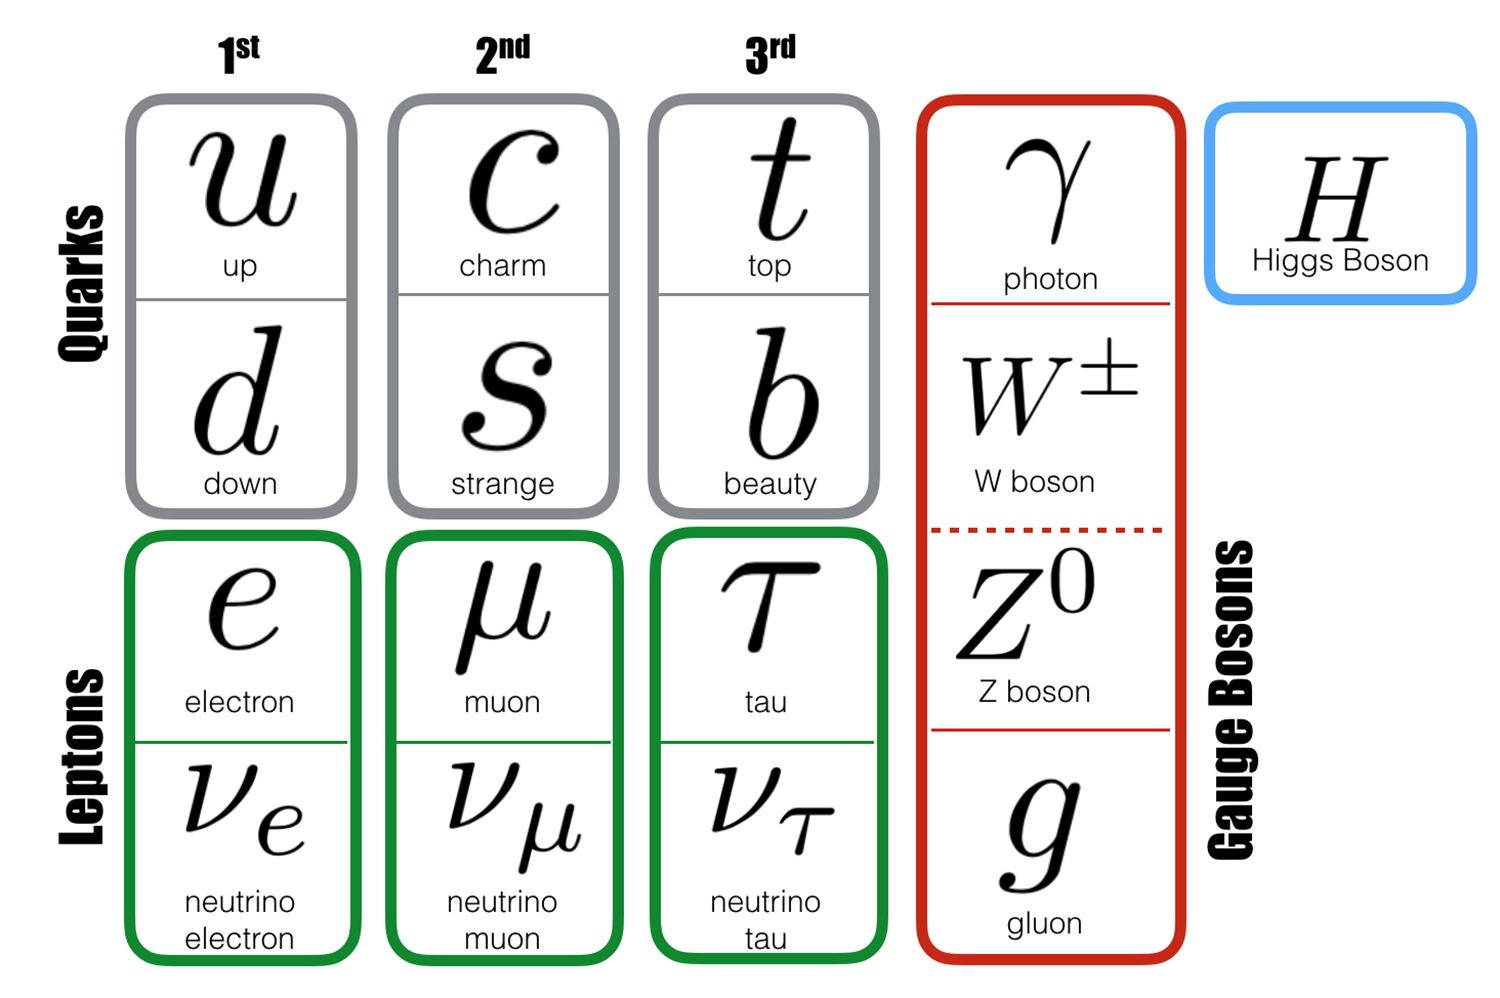
\includegraphics[width = 6 cm]{plots/SM.png}
	\end{figure}
 
	
	Quantum Field Theory describing physics at the TeV scale
	
	\begin{itemize}
		\item Fermions composing matter (leptons and quarks)
		\item Bosons as mediators of the interactions
		\item Scalar Higgs generating mass
	\end{itemize}	
	
\end{frame}

% LHC physics
\begin{frame}
	
	\frametitle{QCD in a nutshell}
	\framesubtitle{LHC physics}
	
	\begin{figure}
		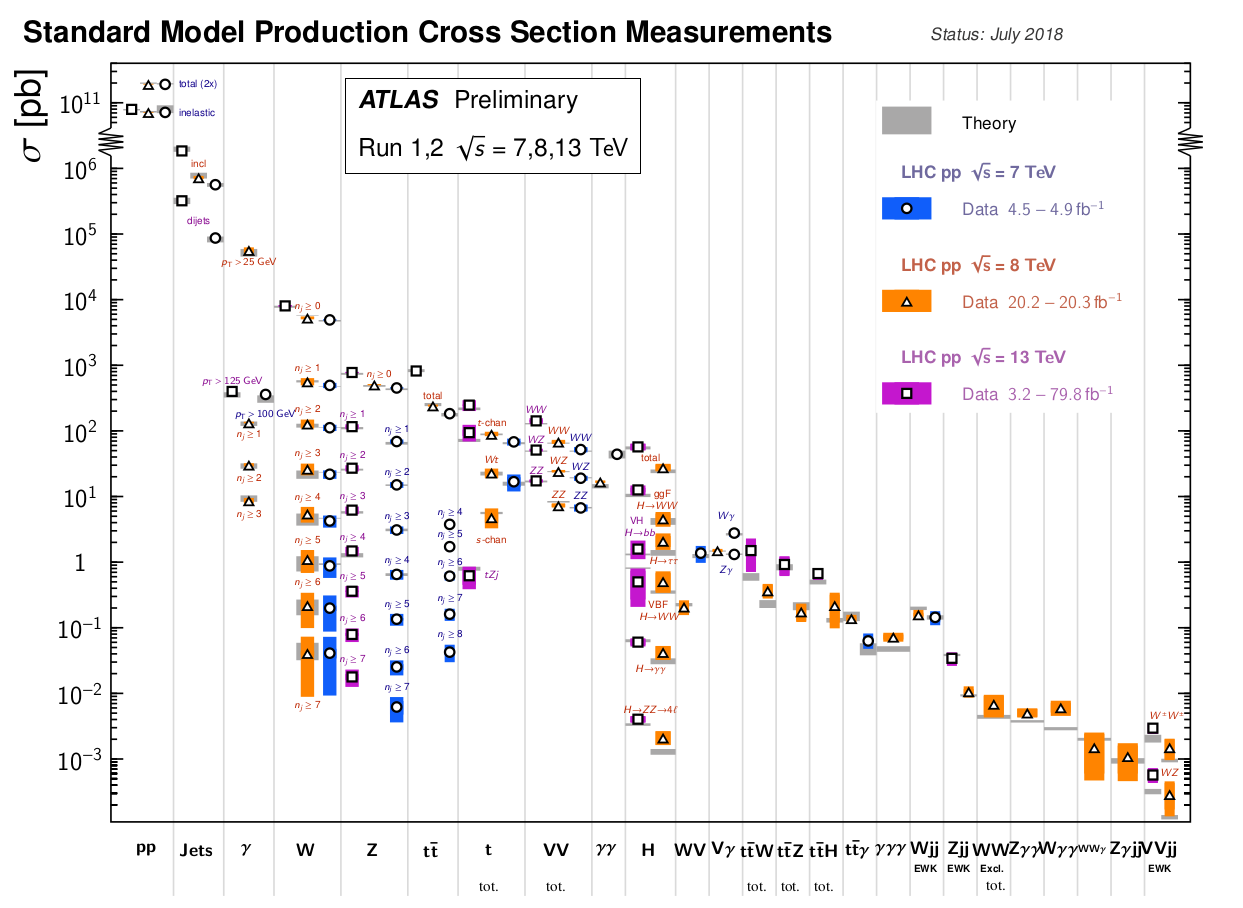
\includegraphics[width = 9.5 cm]{plots/lhc_measurements.png}
	\end{figure}

\end{frame}

% Explore the proton structure
\begin{frame}

	\frametitle{QCD in a nutshell}
	\framesubtitle{Explore the strong interactions}
	
	How to explore proton's inner structure?
	
	\begin{figure}
		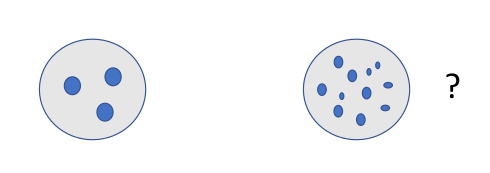
\includegraphics[width = 0.5\linewidth]{plots/protons.png}
	\end{figure}
	
	
	\begin{itemize}
		\item Point-like projectile on the object $\longrightarrow$ DIS
		\item Smash the two objects $\longrightarrow$ LHC physics
	\end{itemize}
	
	{\color{blue}"A way to analyze high energy collisions is to consider any hadron as a composition of point-like constituents $\longrightarrow$ \textbf{partons"} } R.Feynman, 1969 

\end{frame}

% Factorization theorem
\begin{frame}

\frametitle{QCD in a nutshell}
\framesubtitle{Factorization theorem}

\begin{figure}
	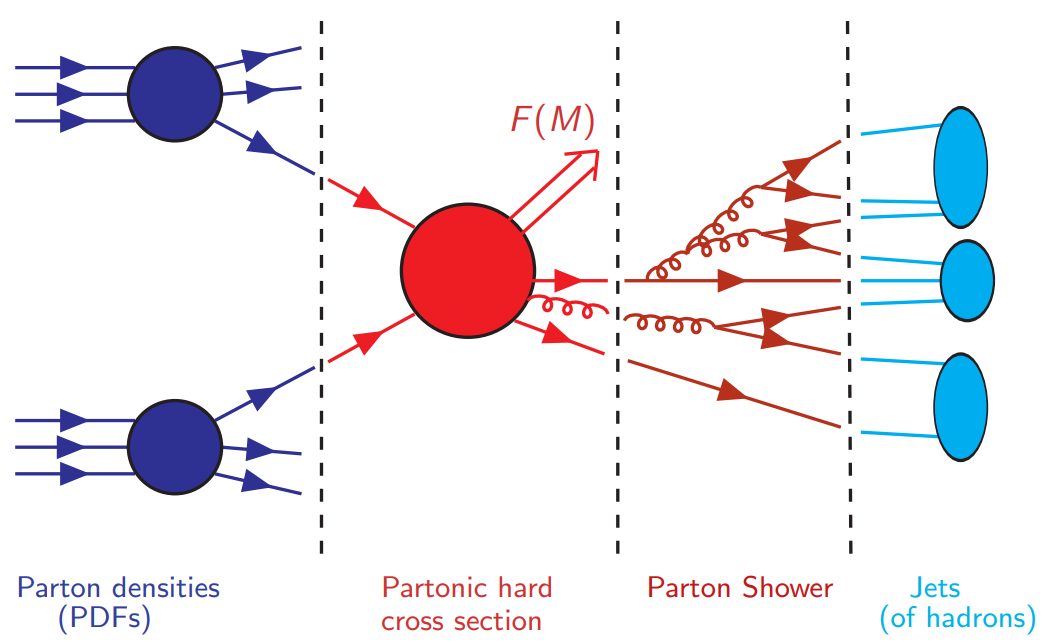
\includegraphics[width = 7 cm]{plots/factorization_1.png}
\end{figure}

Compute cross sections is a {\color{red}hard problem} $\longrightarrow$ {\color{blue} QCD Factorization}

\begin{equation}
	\sigma^{\textrm{F}}(p_{1}, p_{2}) =
	\int_{0}^{1} dx_{1} dx_{2} \; {\color{blue} f_{\alpha}(x_{1}, \mu_{F}^{2}) \ast f_{\beta}(x_{2}, \mu_{F}^{2})}
	\; \ast \;  
	{\color{red}\hat{\sigma}^{\textrm{F}}_{\alpha \beta}(x_{1}p_{1}, x_{2}p_{2}, \alpha_{s}(\mu_{R}^{2}), \mu_{F}^{2})} \nonumber
\end{equation}

\end{frame}

% Machine Learning introduction
\begin{frame}

	\frametitle{Machine learning}
	\framesubtitle{What is Machine Learning?}
	\begin{columns}
		
		\column{0.45\textwidth}
		
		\begin{enumerate}
			\item A subset of Artificial Intelligence (AI) algorithms 
			\item Used to solve \textit{complex} tasks like classification and regression
			\item Rely on comparison with data $\longrightarrow$ {\color{red}Learning} through minimization of some loss
		\end{enumerate}
		
		\column{0.45\textwidth}
		\begin{figure}[!htb]
			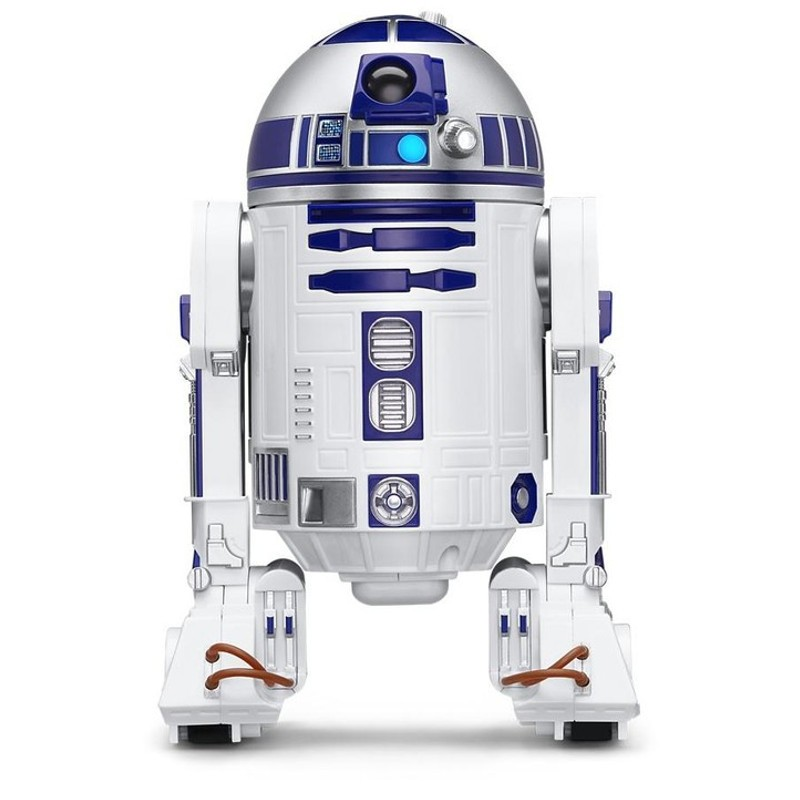
\includegraphics[width = \linewidth]{plots/r2d2.jpeg}
		\end{figure}
	
	\end{columns}

\end{frame}

% N3PDF methodology
\begin{frame}

	\frametitle{The N3PDF project}
	\framesubtitle{Machine Learning for subnuclear structure}

	\begin{enumerate}
		\item Take the asymptotics of $\hat{\sigma}(N)$ computed by following \href{https://arxiv.org/abs/1303.3590}{{\color{blue}1303.3590}} as input (training) data.
		\item Assume the points are sampled from a Gaussian distribution $f(x) \sim N(\mu, K(\Theta, x, x'))$.
		\item Train $\Theta$ by minimizing a $\chi^{2}(f(x)|\Theta, x)$ to guess the underlying law through exhaustive search $\longrightarrow$ {\color{blue}hyperoptimization}
		\item Use the Mellin-space exact coefficient functions computed by \href{https://www.ge.infn.it/~bonvini/higgs/}{{\color{blue}ggHiggs}} as true values for testing and validation.
	\end{enumerate}

\end{frame}

% Results
\begin{frame}

	\frametitle{Results}
	\framesubtitle{Learning a physical quantity}
	
	\begin{figure}
		\minipage{0.32\textwidth}
		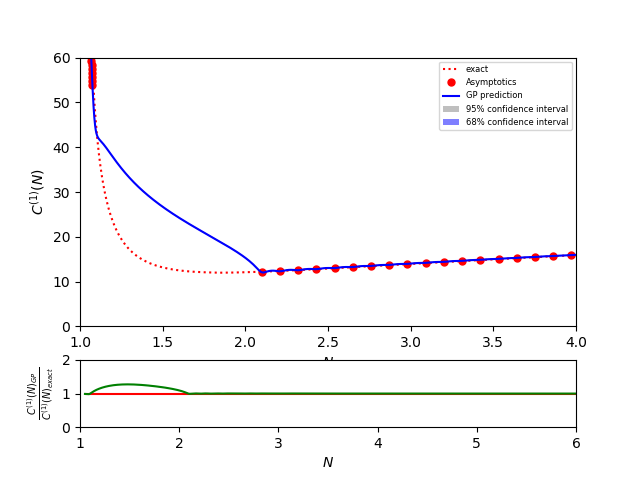
\includegraphics[width = \linewidth]{plots/nlo_test_rquad.png}
		\endminipage\hfill
		\minipage{0.32\textwidth}
		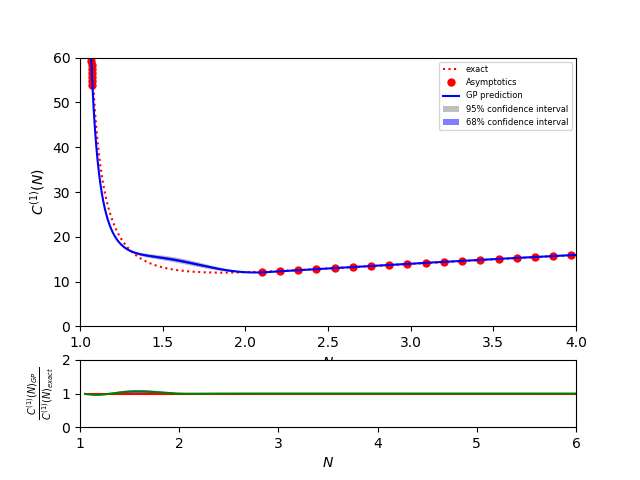
\includegraphics[width = \linewidth]{plots/nlo_test_matern.png}
		\endminipage\hfill
		\minipage{0.32\textwidth}
		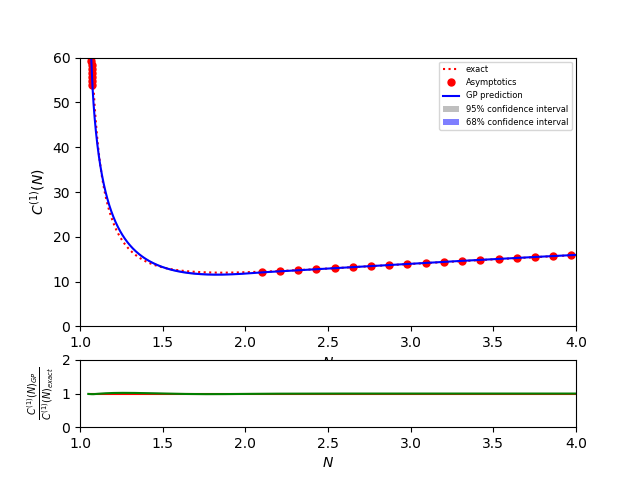
\includegraphics[width = \linewidth]{plots/nlo_matern1.png}
		\endminipage
	\end{figure}
	
	\begin{itemize}
		\item Combination of different kernels leads to better fit
		\item Excellent numerical agreement up to N3LO
	\end{itemize}
	
	{\color{blue}When there is not theory prediction to compare to, use GP approach to estimate theory uncertainty}

\end{frame}

% Conclusions
\begin{frame}
	
	\frametitle{Summary $\&$ Conclusions}

	\vspace{2.0 cm}
	
	\begin{enumerate}
		\item Precise predictions are required towards precision era of the LHC
		\item ML provides an effective way of fitting a curve
		\item Kernel-based methods particularly powerful for interpolation
		\item Theory uncertainty can be extracted from the confidence interval given by the Gaussian Process
	\end{enumerate}

	\vspace{2.0 cm}

	{\small \color{blue} This project has received funding from the European Union$'$s Horizon 2020 research and innovation program under grant agreement No 740006.}

\end{frame}

\end{document}